\chapter{Conclusions and Further Work}
\label{ch:conclusion}
This final chapter summarises the conclusions that can be drawn from the
results presented in this thesis and gives some ideas for directing further
research.

\section{Summary Conclusions}
This thesis has introduced the use of policy gradient reinforcement learning
algorithms in modelling strategies of electricity market participants. Over
the last two decades, competitive markets have become an essential component of
electricity supply industries in many large countries.  They will play an
important role in the future as the world population continues to grow and
finite primary energy fuel resources become increasingly scarce.  Electric
energy trade requires a unique market design, but radical architecture changes
can not be experimented with on real systems.

Computational simulation is a well established technique for evaluating market
design concepts and agent-based simulation is an approach that allows large
complex systems to be modelled.  There are many examples of learning algorithms
being used to model electricity market participants in the literature, but
policy gradient methods have not been previously applied.  These
methods use function approximation techniques to operate in environments
with state and actions spaces that are continuous, discrete or mixed and have
been successfully applied in robot control and other problems.

To examine the properties of policy gradient methods and compare their
performance with previously applied value function based methods, a modular
simulation framework has been defined and implemented.  The framework uses a
power exchange auction market model with nodal marginal pricing to provide an
environment in which agents can \textit{learn to trade power} competitively.

The framework has first been used in a simulation that compares the convergence
to Nash equilibria of four different learning algorithms.  The simulation
structures reproduced the findings of \citeA{krause:nash06} and presented
similar results for policy gradient methods.  Policy gradient methods were
found: to exhibit very different characteristics to value function based
methods, to require a larger number of interactions before learning an optimal
policy and to require low learning rate and exploration rate decay parameters
for complex equilibria to be approached.

In a second simulation the framework was used to compare the same algorithms in
a complex dynamic electricity trading environment.  A reference electric power
system model, designed for reliability analysis, was used to provide a
realistic environment of a reasonable size.  The algorithms were compared in
their ability to observe and exploit constraints in the system as loads followed
an hourly profile.  It was not found that policy gradient methods could use
additional bus voltage data to achieve greater performance than a action-value
function based method or a stateful variant of the Roth-Erev technique.
However, they were shown to learn effective strategies under noisy dynamic
conditions and to improve performance using complex continuous state
representations.

In conclusion, policy gradient methods are a valid option for modelling the
strategies of electricity market participants.  They can use profit feedback
from an electricity market model to adjust the parameters of a policy function
approximator in the direction of increased reward.  Function approximators allow
market participants to be modelled using agents that accept complex power system
state data and produce offers for diverse portfolios of generators with
price markups applied and capacity withheld.  This thesis has compared
a selection of techniques for participant modelling and provides guidance for
algorithm and parameter selection.
% It has been how even moderately complex electricity market simulations produce
% state and action spaces that are too large for value function based methods to
% explore. Policy gradient methods have been shown to produce consistent
% behaviour in increasingly complex dynamic trading problems.
Further development of the ideas in this thesis could allow advanced learning
algorithms to be used to support the decisions made by traders in electricity
markets or in fully automated energy trade.

\section{Further Work}
\label{sec:furtherwork}
This final section highlights some of the shortcomings of the methodology
presented in this thesis and explains how the models could be further
developed. It introduces some alternative learning algorithms that might also be used to
simulate electricity market participant behaviour.
% Also, two new reinforcement learning problem formulations are defined that
% concern two highly pertinent issues in electric power Engineering.
It explains is how a model formulated using data from National Grid
Ltd.~could be used in practical simulations of the UK electricity market and
describes some other possibilities for using AC optimal power flow in
agent-based electric power market simulation.

\subsection{Parameter Sensitivity and Delayed Reward}
The simulations presented in this thesis use typical algorithm parameters that
are either the default values from PyBrain or inspired by the literature. No
study of parameter sensitivity is performed and alternative function
approximation and back-propagation techniques could also be investigated. In
reinforcement learning, parameter sensitivity analysis is often conducted by the
algorithm developers using standard benchmark problems (such as mazes or pole
balancing problems \cite{schaul:2010}) that are familiar to researchers in
artificial intelligence and allow results to be compared. The shortage of
published results and lack of standardised electricity trading models might
limit the benefits of using this problem for general parameter sensitivity
analysis.

The reward signals received by agents in all of the simulations presented in
this thesis result directly from the agent's previous action.  In
practice, a market settlement process would introduce delays to payments for
electricity production. Time did not permit value function based methods with
eligibility traces (See Section \ref{sec:eligibility}) to be compared with
policy gradient methods, but the ability to learn under delayed reward is a
fundamental part of both reinforcement learning and market trade and deserves
investigation in this context.

% Actions in previous states not only effect the reward signal, but the current
% range of possible actions.  The rate at which generator types can ramp up or
% ramp down production is a typical constraining factor in this regard.
% Multi-period optimal power flow formulations may incorporate such constraints,
% but are challenging to implement and solve.

\subsection{Alternative Learning Algorithms}
This thesis has concentrated on traditional value function based methods, the
Roth-Erev technique and two policy gradient reinforcement learning methods.
However, there are other learning algorithms that have been published recently
that could also be used in electric power trade simulations.

\citeA{riedmiller05nfq} presented Neuro-Fitted Q-Iteration (NFQ)
algorithms that attempt to overcome many of the problems experienced when implementing
Q-learning methods with value function approximation using neural networks.
They store all transition experiences and perform off-line updates using
supervised learning techniques such as RProp \cite{riedmiller93}.  The method
has been shown to be robust against parameterisation and to learn quickly in
standard benchmark tests and real-world applications \cite{kietzmann09}.

The GQ$(\lambda)$ algorithm by \citeA{maei10} is another extension of Q-learning
for operation in continuous environments.  Convergence guarantees have been
shown and the scaling properties suggest the method is suitable for large-scale
reinforcement learning applications.
% A software implementation of GQ$(\lambda)$
% has been developed and recently made available as open source.

Four new Natural Actor-Critic algorithms have been presented by
\citeA{bhatnagar09}. Like ENAC, they use function approximation techniques and
are suitable for large-scale applications of reinforcement learning.  Three of
the algorithms are extensions to ENAC, but are fully incremental: the gradient
computation is never reset while the policy is updated at every simulation step.
 The authors state a need to assess the ultimate utility of these algorithms
through application in real-world problems.

This thesis provides a framework that would allow implementations of these
algorithms to be assessed and used to research aspects of electricity
markets.

% \subsection{Learning to Optimise Power Flow}
% Two important problems in electric power Engineering, to which to the
% application of advanced reinforcement learning algorithms would be of value,
% are:
% \begin{itemize}
%   \item System optimisation, close to real-time, such that sufficient reserve
%   is allocated to ensure acceptable system security while costs are minimised
%   according to the outcome of the electricity markets, and
%   \item Capital investment planning, both by system operators needing to expand
%   transmission capacity and energy companies wanting to develop new generating
%   plant.
% \end{itemize}
%
%
% As explained in Section \ref{sec:opf}, the objective of the classical optimal
% power flow problem is to find generator set-points that allow all system and
% plant constraints to be satisfied while the total system cost is minimised.
% Interior point methods are possibly the most robust technique for finding
% solutions, but the problem may also be formulated as a continuous
% reinforcement learning task that could be learned by a system operator agent.
% To illustrate the concept, this section presents a preliminary formulation of
% such a task and demonstrates how a system operator agent can use policy
% gradient methods to learn to optimise power flow.
%
% \subsubsection{System Operator Task and Environment}
% The state of the system operator agent's environment is defined simply as a
% demand forecast.  That is, the environment returns a vector of active power
% demand at all system buses.  The initial demand is assumed to be peak and is
% used to normalise the values of the sensor vector to be between $-1$ and $+1$
% before input the the mutil-layer perceptron used for policy function
% approximation.  Simulations are divided into episodes (days) over which the
% demand at each bus follows the profile shown in Figure X.
%
% The agent's action and the output of the policy function approximator is a
% vector of the active power set-points of all generators, excluding the
% generator at the system slack bus.  The set-points are bound by the generator's minimum
% and maximum rated capacity. These bounds are used to denormalise the output
% values from the final Sigmoid layer (that are between $-1$ and $+1$) to give
% valid set-point values.
%
% The new generator set-points are used to form an AC power flow problem that is
% solved using Newton's method \cite{tinney:67}.  The power flow solution
% determines the complex voltage at each bus, the branch power flows and losses,
% the reactive power output of the generators and the active power output of the
% slack bus generator.
%
% The reward is defined as the negative of the sum of all generator costs.  The
% negative of the costs must used since the learning methods attempt to maximise
% reward and the objective is to minimise cost.  The power flow solution does not
% satisfy system constraints, such as voltage limits or generators reactive power
% limits and penalty costs must be applied to the reward so the agent learns to
% obey them.
%
% \subsubsection{Slack Bus Generator Control}
% This initial proof of concept attempts only to enforce the set-point limit on
% the slack bus generator.  The reward is updated according to
% \begin{equation}
% r =
% \begin{cases}
% r + \phi (P_{slack} - P_{max}), & \text{$P_{slack} > P_{max}$} \\
% r, & \text{otherwise}
% \end{cases}
% \end{equation}
% The six bus network model described in Chapter \ref{ch:nashanalysis} is used
% with the coefficients of the generator's quadratic cost functions given in Table X.  Learning is conducted in batch
% mode, with 7 episodes conducted before the parameters of the policy are
% updated.  The system operator agent uses the ENAC learning method with RProp
% gradient descent and an initial value of $\sigma = 50$, which is reduced after
% each simulated week according to $\sigma_{i+1} = 0.5\sigma_i - 2$.
%
% Figure X shows the average output of each generator over 52 simulated weeks of
% control. Plotted in Figure Y is the average total system cost for each week along with
% theoretically optimal values as calcualted by DC and AC optimal power flow
% solvers.  The results show that, with suitable initial experimentation, the
% agent learns to dispatch the generators in the most economically efficient
% manner while controlling the slack bus generators to valid output levels.  The
% average total system cost converges to slightly less that of the optimal
% solution due to the disregard for other constraints, particularly the
% branch flow constraint between buses 2 and 4 which is binding at times of peak
% load.
%
% \subsection{Learning to Plan Investment}

\subsection{UK Transmission System}
Some of the more ambitious agent-based electricity market simulations have used
stylised models of national transmission systems
\cite{cincotti:09,weidlich:06}.  This work has often been motivated by recent
or expected changes to the arrangements in the associated regions.
% The drop in
% oil prices around the time of the global economic crash in 2008 was not
% reflected quickly in energy prices and this amplified concerns over liquiduty
% levels in the UK electricity markets.  Ofgem found competition to be
% sufficient[ref], but the concerns persists and the market arrangements have
% been re-examined under Project Discovery[ref].
In the UK, nine large power stations are due to be decommissioned by 2016 in
accordance with EU Large Combustion Plant Directive \cite{ngt07lcpd}.  Coupled
with obligations, made in the Climate Change Act 2008, to cut greenhouse gas
emissions by 80\% of 1990 levels by 2050, coming years are likely to see major
changes in the way the UK power system is operated.
% The ability of the market to sufficiently incentivize new
% investment in generation that will cover the resulting shortfall is in question.  The concern extends
% to the need for long-term investment in new nuclear power plant that is deemed
% necessary for the UK to meet the legally binding obligations, made in the
% Climate Change Bill, to cut greenhouse gas emissions by 80\% by 2050, compared
% to 1990 levels.
Examination of the situation could be enhanced by advanced participant
behavioural models and accurate electric power system simulations such as those
presented in this thesis.

Figure \ref{fig:ngt_grid} illustrates a model of the UK transmission system that
has been formulated from data provided by the \citeA{ngtsys2010}.  This model
has been converted into PSS/E raw file format and is included with the
code developed for this thesis (See Appendix \ref{sec:pylon}).
% Generator set-points were determined using the state estimator from Pylon
% [Crow].  The power flow results are shown in Figure X and correlate accurately
% with those in [SYS], having a mean variance of X.XX. Cost data for each of the
% aggregated generating units has been estimated from public sources and stored
% in the PSS/E version 30 optimal power flow data file in Appendix
% \ref{sec:nget_opf}.  Execution times for solving this case using DC, AC and
% unit de-commitment optimal power flow are shown in Table X.
\ifthenelse{\boolean{includefigures}}{
	\begin{figure}
	  \centering
	  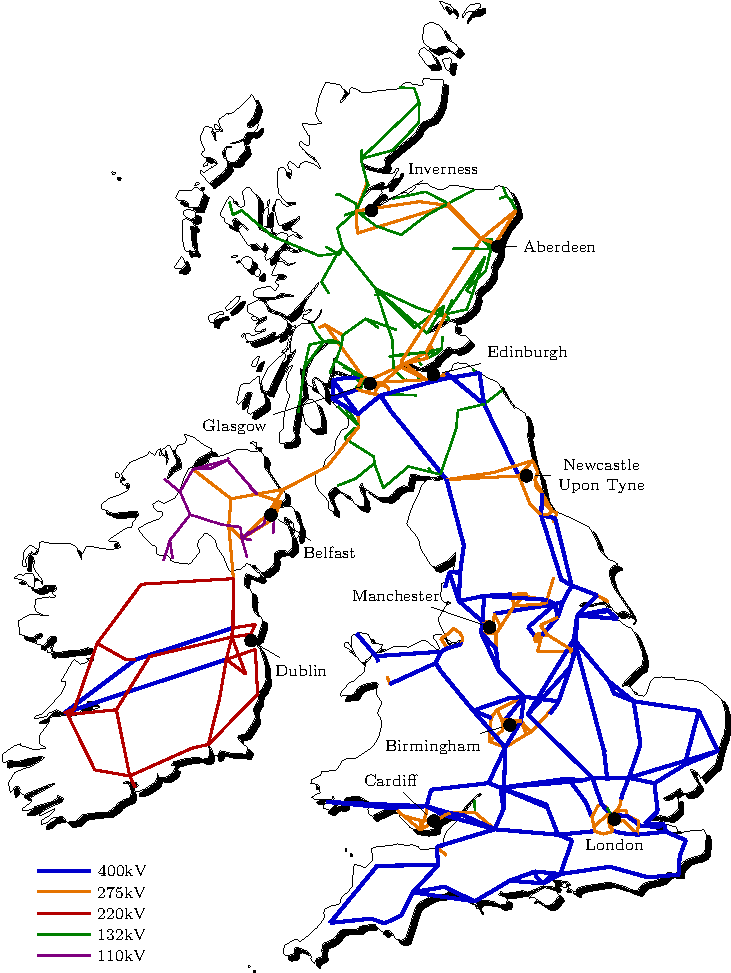
\includegraphics{figures/ngt_grid}
	  \caption{UK transmission system.}
	  \label{fig:ngt_grid}
	\end{figure}
}{}
It is currently too computationally expensive to be solved repeatedly in an
agent-based simulation, but optimisation efforts might allow for it to be used
in studies pertinent to the UK energy industry.

% However, significant improvements in
% speed should be possible through more efficient construction of the Hessian
% matrices in the AC optimal power flow solver.  Agent-based simulation lends
% itself to parallelisation and the artificial neural networks could be
% processed in multiple threads on multi-core processors or on distributed
% memory architectures.

\subsection{AC Optimal Power Flow}
This thesis presents the first application of AC optimal power flow in
electricity market simulation using reinforcement learning agents.  AC optimal
power flow formulations are more difficult to implement and more computationally
expensive to solve than their linearised DC counterparts.  The
additional time and effort required for their use does not always add sufficient
value to simulations.  However, the option to use AC formulations does
provide certain opportunities for further work.

The inclusion of reactive power costs in the objective function of an AC optimal
power flow problem provides an opportunity to run auctions for voltage support
in parallel with those for active power.  These could be open to agents
associated with reactive compensation equipment such as that commonly needed for
wind farm developments.  Traditionally, reactive power markets have been mostly
of academic interest, but as the UK makes greater use of on and off-shore wind
power, the topic could become of increasing importance.

Bus voltages are not all assumed to be 1~per-unit in AC optimal power flow
problems, but are part of the vector of optimisation variables.  Adjusting
phase shift angles, $\theta_{shift}$, can offer a degree of control over
the direction of power flows.  The control of transformer tap ratios, $\tau$,
and phase shift angles by learning agents could become a topic of interest
in congestion management research.

\subsection{Multi-Market Simulation}
% Policy gradient method's superior use of sensory data and their ability to
% operate in large action domains opens opportunities for more detailed study of
% inter-market relationships.
Finally, the global economy is a holistic system of
systems and the analysis of markets independently must be of limited value.
Recent agent-based electricity market studies have investigated the
interaction between electricity, gas and emission allowance markets
\cite{krause:gas,wang:09}.
% Non-linear models [ref] have been published for gas flows in pipelines such as
% those of the UK gas network.

Data for the UK gas transmission network provided by the \citeA{ngtsys2010} is
of limited detail, compared to that for the electricity transmission system,
but suitable models could be used to study the the relationships
between UK gas and electricity markets.  As in \citeA{krause:gas}, actions in
the gas market would constrain the generators options to sell power in subsequent
electricity auctions.  Add to this the option to trade in emissions allowance
markets and agents would be presented with large state and action spaces and
would require suitably advanced learning methods.

% \subsection{Common Information Model}
% Many tools exist for steady-state analysis of balanced three-phase AC networks
% and most are centred around bespoke models that describe the power system
% data.  Several attempts have been made in the past to standardise the format
% in which power system data is stored [CDF, UKGDS, ODF] and latest and most
% popular is the Common Information Model.
%
% The Common Information Model (CIM) is an abstract ontological model that
% describes the elements of national electric power systems and the associations
% between them.  CIM is an evolving international standard approved by the
% International Electrotechnical Commission (IEC).
%
% Unlike many tool specific models the CIM does not simplify the power system
% into a graph of buses connected by branches.  Instead it describes each of the
% components in the system and the electrical connectivity between them.
% Conventional numerical techniques for steady-state analysis of AC power
% systems require a simplified bus-branch model such that when the voltage angle
% and magnitude at each bus is determined the power flows on each branch may be
% calculated.

% market power, constraint management
%\section{Decentralised Trade}
% distribution level, renewables
%\section{Standarisation}
% CIM for markets
%\section{Blackbox optimisation}
% periodic

%\subsection{Summary}